\documentclass[runningheads]{llncs}

% ── Core packages ──────────────────────────────────────────────────────────────
\usepackage[T1]{fontenc}
\usepackage{graphicx}
\usepackage{amsmath,amssymb}
\usepackage{booktabs}
\usepackage{multirow}
\usepackage{multicol}
\usepackage{tabularx}
\usepackage[table,dvipsnames]{xcolor}
\usepackage{pgfplots}
\usepackage{tikz}
\usetikzlibrary{shapes.geometric,arrows.meta,positioning,fit,backgrounds}
\usepackage{algorithm}
\usepackage{algorithmic}
\usepackage[hidelinks]{hyperref}
\usepackage{url}
\usepackage{natbib}
\usepackage{microtype}      % better justification
\usepackage{float}
\usepackage{placeins}       % \FloatBarrier
\pgfplotsset{compat=1.18}
\def\UrlFont{\rmfamily}

% ── Spacing helpers ─────────────────────────────────────────────────────────────
\setlength{\textfloatsep}{8pt plus 2pt minus 2pt}
\setlength{\floatsep}{6pt plus 2pt minus 2pt}
\setlength{\intextsep}{6pt plus 2pt minus 2pt}
\setlength{\abovecaptionskip}{4pt}
\setlength{\belowcaptionskip}{2pt}

% ── Colour palette for heatmap ──────────────────────────────────────────────────
\definecolor{hBlue}{RGB}{198,219,239}
\definecolor{hGreen}{RGB}{186,228,179}
\definecolor{hYellow}{RGB}{254,217,142}
\definecolor{hOrange}{RGB}{253,174,107}
\definecolor{hRed}{RGB}{240,159,140}
\definecolor{hGray}{RGB}{220,220,220}

% ───────────────────────────────────────────────────────────────────────────────
\begin{document}

\title{Constraints and Heuristics: Leveraging Dataset Metadata for Efficient AutoML}
\titlerunning{Constraints and Heuristics for Efficient AutoML}

\author{Harsh Kakadiya\inst{1} \and
        Juli Kyada\inst{1}    \and
        Kaushal Savaliya\inst{1} \and
        Jalpesh Vasa\inst{1}}
\authorrunning{Harsh Kakadiya et al.}

\institute{Department of Artificial Intelligence and Machine Learning,\\
           Chandubhai S.\ Patel Institute of Technology (CSPIT),\\
           Faculty of Technology and Engineering,\\
           Charotar University of Science and Technology (CHARUSAT),\\
           Changa, Gujarat, India\\
           \email{harshkakadiya128@gmail.com, julikyada293@gmail.com, kaushalsavaliya2627@gmail.com, jalpeshvasa.it@charusat.ac.in}}

\maketitle

% ══════════════════════════════════════════════════════════════════════════════
\begin{abstract}
This work presents MetaFlow, a metadata-driven AutoML framework that uses lightweight dataset profiles (sample size, feature types, imbalance, cardinality, and outlier density) to deterministically prune and re-rank candidate pipelines before training. Unlike black-box optimization systems that rely on extensive trial-and-error, MetaFlow encodes concise, interpretable rules to avoid evaluating clearly unsuitable learners, reducing compute by pruning the search space (reported here as $\sim$67\%). The primary contribution is a practical "grey-box" approach that trades exhaustive search breadth for targeted efficiency using human-interpretable constraints and prioritization.

It is emphasized that MetaFlow is complementary to, rather than a replacement for, modern AutoML toolkits: it is intended to provide inexpensive, data-driven pruning and warm-start guidance, which can be combined with Auto-sklearn, FLAML, or other optimizers. Limitations are also highlighted: the rule thresholds (e.g., categorical cut-offs, missingness) are heuristic and dataset-dependent, and the empirical study focuses on representative tabular cases rather than an exhaustive benchmark. A reproducibility checklist and a benchmarking protocol are described to facilitate direct comparison with state-of-the-art AutoML systems.

\keywords{AutoML \and metadata \and pipeline selection \and meta-learning \and algorithm selection \and data profiling \and preprocessing}
\end{abstract}

% ══════════════════════════════════════════════════════════════════════════════
\section{Introduction}
\label{sec:intro}

Designing effective machine learning pipelines encompassing data cleaning,
feature engineering, algorithm selection, and hyperparameter tuning demands
substantial domain expertise and computational effort.
AutoML systems address this challenge by automating the search over pipeline
configurations.  Auto-WEKA~\cite{thornton2013auto} first formalised the
\emph{Combined Algorithm Selection and Hyperparameter} (CASH) problem, while
Auto-sklearn~\cite{feurer2015efficient} introduced meta learning and
warm-starting.  Contemporary methods employ Bayesian
optimisation~\cite{bergstra2011algorithms}, genetic
programming~\cite{olson2016tpot}, and random
search~\cite{li2017hyperband} powerful but computationally intensive approaches
  that often evaluate many unsuitable candidates before converging.

An alternative approach relies on dataset \emph{metadata} comprising structural and statistical properties to warm-start or constrain the search space via a complementary paradigm~\cite{leite2012survey}. Dataset attributes such as sample size, feature types, missingness, outlier density, and class imbalance can guide an automated system to discard unsuitable algorithms \emph{before} training begins~\cite{wang2021flaml}. This work presents an end-to-end framework named \textbf{MetaFlow} that extracts metadata and leverages it to automatically detect task types, apply target transformations, prioritize candidate models, and evaluate pipelines without exhaustive search. The investigation is guided by two primary research questions: \textbf{RQ1 (Efficacy):} Can lightweight dataset metadata accurately detect task types and rank appropriate learning algorithms? \textbf{RQ2 (Efficiency):} Does metadata-based pruning substantially reduce computational cost compared to exhaustive selection?

% ══════════════════════════════════════════════════════════════════════════════
\section{Related Work}
\label{sec:related}

The CASH problem formalizes the joint search over algorithms and hyperparameters. Auto-WEKA~\cite{thornton2013auto} pioneered Bayesian optimization (SMAC/TPE) for this hierarchical space, requiring many expensive black-box evaluations. TPOT~\cite{olson2016tpot} employs genetic programming to evolve flexible pipeline structures, though at high computational cost. FLAML~\cite{wang2021flaml} and LightAutoML propose frugal optimization strategies that prioritize low-cost learners, yet these frameworks still rely on empirical trial-and-error rather than \emph{a priori} dataset reasoning.

Meta-learning frames algorithm selection as supervised learning over prior experimental results. Auto-sklearn~\cite{feurer2015efficient} advances this via warm-starting from a meta-knowledge repository (OpenML~\cite{vanschoren2013openml}), using statistical, information-theoretic, and landmarking meta-features~\cite{leite2012survey}. Although effective, this approach requires large, computationally expensive-to-maintain offline repositories.

Beyond algorithm choice, metadata also governs preprocessing decisions. High-cardinality categoricals often necessitate target encoding rather than one-hot encoding, and imputation strategies can affect downstream performance more than classifier choice~\cite{li2021cleanml}.

\subsection{Domain-Specific Implementations}
Domain-specific machine learning methodologies have achieved notable success in specialized tasks, including solar power forecasting \cite{dhaked2023power, dhaked2025exploring}, wind turbine pitch control \cite{narayanan2024improved}, medical cyber-physical systems \cite{dhaked2025recent}, epidemic forecasting \cite{dhaked2025prediction}, and power grid contingency ranking \cite{dhaked2025ensemble}. However, these applications rely on customized, manually designed pipelines. This underscores the need for generalized, metadata-driven AutoML frameworks that can automatically select suitable models based on dataset properties.

\subsection{Research Gap and Contribution}
A gap exists between pure optimization (which is general but slow) and pure meta-learning (which requires massive training logs). Existing systems rely on metadata for initialization only, then perform black-box search, and few frameworks employ \emph{hard constraints} to deterministically prune the search space. MetaFlow bridges this gap with a ``grey-box'' technique: the matching of interpretable metadata is performed directly to pipeline decisions using a rule-based expert system, which casts out inappropriate candidates \emph{before} training begins~\cite{hutter2019automated}.

Compared to contemporary AutoML, systems like Auto-sklearn use meta-features for warm-starting optimization~\cite{feurer2015efficient}, while FLAML prioritizes low-cost learners to trade accuracy for speed~\cite{wang2021flaml}. However, both methods still run numerous evaluations. By contrast, MetaFlow places deterministic, interpretable constraints at the front of the pipeline, pruning unsuitable models under transparent rules. This makes MetaFlow complementary: it narrows the search space using heuristics and hands the reduced pool to downstream optimizers for tuning.

% ══════════════════════════════════════════════════════════════════════════════
\section{Methodology}
\label{sec:methodology}

MetaFlow is an end-to-end system that extracts structural and statistical
metadata from a tabular dataset and uses it to drive every downstream
decision   task detection, preprocessing, model selection, and evaluation  
without exhaustive search. Figure~\ref{fig:metaflow} summarises the processing
stages.

% ── Formal problem statement ─────────────────────────────────────────────────
\subsection{Formal Problem Statement}

Let a dataset be denoted by $\mathcal{D}=(X,y)$ with $X\in\mathbb{R}^{n\times p}$
and target $y$.  The \emph{metadata extractor} is a deterministic mapping
\begin{equation}
  M:\;\mathcal{D} \mapsto m,\qquad m\in\mathcal{M},
\end{equation}
where $m$ is a structured metadata object (cardinality, missingness, $p/n$,
skewness, etc.).  A rule-based selector is a function
\begin{equation}
  R:\;\mathcal{M} \mapsto \mathcal{G},
\end{equation}
that maps metadata to a candidate model pool $\mathcal{G}=\{g_1,\dots,g_L\}$ and
associated hyperparameter grids.  A pruning operator $P$ deterministically
removes unsuitable candidates given thresholds and hard constraints:
\begin{equation}
  \mathcal{G}' = P(\mathcal{G}, m),\qquad \mathcal{G}'\subseteq\mathcal{G}.
\end{equation}
Each candidate pipeline $\pi$ in $\mathcal{G}'$ is evaluated using a
cross-validation evaluator $E$ producing a score $s$ and cost $c$:
\begin{equation}
  (s,c) = E(\pi,\mathcal{D}).
\end{equation}
The final selection chooses the pipeline that maximises a user-specified utility
($\,$e.g. test metric subject to a cost budget):
\begin{equation}
  \pi^* = \arg\max_{\pi\in\mathcal{G}'}\; U\big(E(\pi,\mathcal{D})\big).
\end{equation}

This concise formalisation highlights where metadata-driven rules intervene
prior to any model training and explicitly separates pruning, evaluation, and
selection.

% ── Pipeline figure ───────────────────────────────────────────────────────────
\begin{figure}[t]
\centering
\scalebox{0.78}{
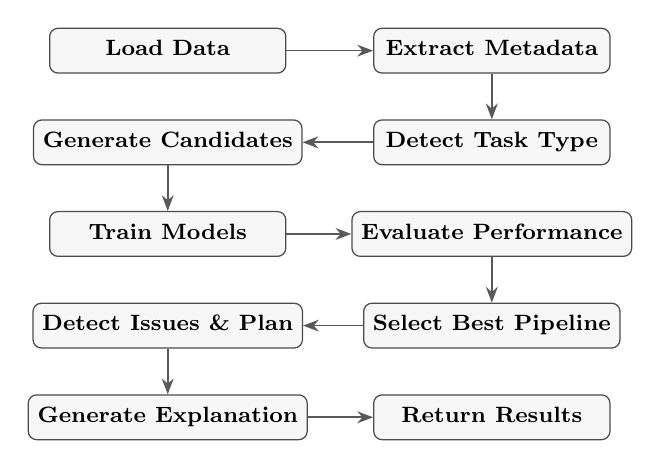
\begin{tikzpicture}[
  node distance=0.35cm and 1.1cm,
  stage/.style={
    rectangle, rounded corners=3pt,
    minimum width=3.0cm, minimum height=0.52cm,
    text centered, draw=black!70, line width=0.45pt,
    fill=gray!6, font=\footnotesize\strut
  },
  arrow/.style={-Stealth, line width=0.6pt, draw=black!65}
]
% Left column
\node[stage] (load)     at (0,0)            {\textbf{Load Data}};
\node[stage] (generate) [below=0.58cm of load]  {\textbf{Generate Candidates}};
\node[stage] (train)    [below=0.58cm of generate] {\textbf{Train Models}};
\node[stage] (issues)   [below=0.58cm of train]   {\textbf{Detect Issues \& Plan}};
\node[stage] (explain)  [below=0.58cm of issues]  {\textbf{Generate Explanation}};
% Right column
\node[stage] (extract)  [right=of load]          {\textbf{Extract Metadata}};
\node[stage] (detect)   [below=0.58cm of extract] {\textbf{Detect Task Type}};
\node[stage] (evaluate) [below=0.58cm of detect]  {\textbf{Evaluate Performance}};
\node[stage] (select)   [below=0.58cm of evaluate]{\textbf{Select Best Pipeline}};
\node[stage] (return)   [below=0.58cm of select]  {\textbf{Return Results}};
% Arrows
\draw[arrow] (load)     -- (extract);
\draw[arrow] (extract)  -- (detect);
\draw[arrow] (detect)   -- (generate);
\draw[arrow] (generate) -- (train);
\draw[arrow] (train)    -- (evaluate);
\draw[arrow] (evaluate) -- (select);
\draw[arrow] (select)   -- (issues);
\draw[arrow] (issues)   -- (explain);
\draw[arrow] (explain)  -- (return);
\end{tikzpicture}
}
\caption{MetaFlow processing stages (left column: pipeline flow; right column: metadata-driven decisions).}
\label{fig:metaflow}
\end{figure}

Rule-based constraints encode simple, domain-informed rejection and
prioritisation rules so that clearly unsuitable algorithms are removed before
any training, saving compute and yielding human-interpretable decisions that
are easier to audit than opaque warm-start priors.

% ── Metadata Extraction ───────────────────────────────────────────────────────
\subsection{Metadata Extraction}

Given feature matrix $X \in \mathbb{R}^{n \times p}$ and target vector $y$, the
\texttt{MetadataExtractor} computes nine metadata groups: (1)~dataset dimensions
$(n,p)$; (2)~feature types, re-classifying numeric columns with
$\leq\!\tau_\text{cat}=10$ unique values as categorical; (3)~target statistics;
(4)~quality profile (per-feature missing ratios, duplicate-row count);
(5)~descriptive statistics (skewness, kurtosis per feature); (6)~outlier profile
via the IQR rule; (7)~cardinality profile; (8)~Pearson correlations with the
target; and (9)~class-imbalance profile, flagging \texttt{is\_highly\_imbalanced}
when any class represents ${<}5\%$ of samples.  This metadata dictionary is the
\emph{sole input} to all subsequent modules, ensuring every decision traces to a
measurable dataset property.
Several internal thresholds are heuristic choices: for example,
$\tau_{\text{cat}}=10$ (reclassifying low-cardinality numerics as categorical)
and $\theta_{\text{miss}}=0.5$ (feature drop threshold). These values were
selected from common practice in applied ML and small-scale internal testing to
produce stable, interpretable behaviour across diverse tabular datasets. Although
such thresholds are dataset-dependent, Section \ref{sec:limitations} discusses
sensitivity, how thresholds can be adapted, and outlines a sensitivity study
as part of a reproducibility checklist.

% ── Task Detection & Preprocessing ───────────────────────────────────────────
\subsection{Task Detection and Preprocessing}

The \texttt{TaskDetector} infers classification vs.\ regression from $y$ via a
rule chain (threshold $\tau_\text{cls}=20$, minimum samples-per-class
$\tau_\text{min}=10$): non-numeric $y \Rightarrow$ classification (conf.\ 1.0);
$|y_u|=2 \Rightarrow$ binary classification (0.95); integer $y$ with
$|y_u|<\tau_\text{cls} \Rightarrow$ multiclass (0.90); $|y_u|>0.5n \Rightarrow$
regression (0.95).

Before any pipeline is trained, \texttt{DataPreprocessor} performs a single pass:
features with missing ratio ${>}\theta_\text{miss}=0.5$ are dropped; remaining
missing values are imputed (median for numeric, mode for categorical); empty rows
and rows with missing target are removed.  Inside each scikit-learn
\texttt{Pipeline}, a \texttt{ColumnTransformer} applies standard scaling to
numerical features and one-hot encoding (\texttt{handle\_unknown=`ignore'}) to
categorical features.  Processed data are reused across all candidate pipelines
for fair comparison.

% ── Rule-Based Model Selection ────────────────────────────────────────────────
\subsection{Rule-Based Model Selection}

The \texttt{RuleBasedModelSelector} mechanism for exhaustive algorithm search is solved by providing rules based on metadata that relate to the size, complexity, class imbalance and cardinality of the data, its density of outliers, and its distributional skewness. Sample count $n$ is binned into five tiers: \emph{tiny} ($<$1\,K), \emph{small} (1\,K--10\,K), \emph{medium} (10\,K--100\,K), \emph{large} (100\,K--1\,M), and \emph{huge} ($\geq$1,M). A complexity score is derived from: high dimensionality ($p>50$, $+2$), high $p/n$ ratio ($>0.1$, $+2$), categorical dominance ($>50\%$, $+1$), and moderately many features ($p>20$, $+1$), mapping to \emph{simple} ($\leq 2$), \emph{moderate} (3--4), or \emph{complex} ($\geq 5$). The size-tiered base model pools for both types of task are shown in Table~\ref{tab:model_rules}.

\begin{table}[t]
\centering
\caption{Model pool by dataset-size tier. Models are selected based on
dataset size and complexity; see text for modifier rules.}
\label{tab:model_rules}
\setlength{\tabcolsep}{4pt}
\small
\begin{tabular}{@{}lp{4.0cm}p{4.0cm}@{}}
\toprule
\textbf{Tier} & \textbf{Classification} & \textbf{Regression} \\
\midrule
Tiny        & LR, DT, RF, NB, Ridge-LR, KNN         & OLS, Ridge, DT, Lasso, ElasticNet, KNN \\[2pt]
Small--Med. & RF, XGB, LGBM, GB, LR, KNN, NB        & RF, XGB, LGBM, GB, Ridge, KNN, SVR \\[2pt]
Large--Huge & LGBM, XGB, GB, LR(SAG), RF, Ridge-LR  & LGBM, XGB, GB, Ridge(SAG), RF, Lasso, SVR \\
\bottomrule
\multicolumn{3}{@{}l}{\scriptsize LR=Logistic Regression, DT=Decision Tree, RF=Random Forest,}\\
\multicolumn{3}{@{}l}{\scriptsize NB=Naive Bayes, KNN=$k$-NN, GB=Gradient Boosting,}\\
\multicolumn{3}{@{}l}{\scriptsize XGB=XGBoost, LGBM=LightGBM, SVR=Support Vector Regressor.}
\end{tabular}
\end{table}

Once the initial list is compiled the modifiers re-rank and add modifiers to the primary list: high dimensionality ($p>50$ or $p/n>0.1$), removes RF, SVM and adds regularised LR (L1/L2); the \texttt{is\_highly\_imbalanced} flag adds the \texttt{class\_weight=`balanced'}; high cardinality categoricals add tree-based models (XGB, LGBM, RF); outlier density~${>}5\%$ adds tree and demotes linear (after increasing precision of tree); skewed targets ($|\gamma_y|>1$), adds tree models (to make them independent of monotone transformation on target).  Each recommendation includes a priority ranking, a human-readable description and a hyperparameter (hp) grid, with the top $k=5$ passed on to pipeline generation.

% ── Training, Evaluation, Selection ──────────────────────────────────────────
\subsection{Training, Evaluation, and Selection}

The dataset is partitioned into an 80\% training split and a 20\% held-out test split, utilizing stratified splitting for classification tasks to maintain target distribution. The optimal set of hyperparameters is obtained by performing a grid search (\texttt{GridSearchCV}) over a predefined parameter space using 5-fold cross-validation (CV) on the training set. For instance, the search grid for Random Forest spans \texttt{n\_estimators} $\in \{50, 100, 200\}$ and \texttt{max\_depth} $\in \{5, 10, \text{None}\}$, while for gradient-boosting algorithms (XGBoost, LightGBM), it spans \texttt{learning\_rate} $\in \{0.01, 0.1\}$ and \texttt{max\_depth} $\in \{3, 6\}$. The best-performing configuration is selected based on mean CV performance (accuracy for classification, $R^2$ for regression), refit on the entire training split, and evaluated on the test split. Evaluation metrics include accuracy, precision, recall, and weighted F1-score for classification, and $R^2$, Mean Squared Error (MSE), Root Mean Squared Error (RMSE), and Mean Absolute Error (MAE) for regression. Performance warnings are automatically raised if the test score falls below 0.70, the generalization gap (train--test difference) exceeds 0.10, or the cross-validation standard deviation $\sigma_{CV}$ exceeds 0.15. The most appropriate pipeline is decided upon based on the top scoring test metric and suggestions for optimization are provided with issues identified.

% ══════════════════════════════════════════════════════════════════════════════
\section{Results}
\label{sec:results}

Evaluation of MetaFlow was conducted on four real-world datasets:
\textbf{D1 (Heart Disease)}~\cite{janosi1988heart} represents a small classification task ($n=1{,}025$, $p=13$, balanced targets with 51.3\% cases). Preprocessing uses median imputation, mode imputation, and scaling.
\textbf{D2 (Credit Fraud)}~\cite{dalpozzolo2015fraud} is a large, highly imbalanced classification task ($n=284{,}807$, $p=30$, 0.17\% minority class). Preprocessing scales the time and amount features.
\textbf{D3 (Brain Cancer)}~\cite{feltes2019cumida} is a high-dimensional multiclass task ($n=130$, $p=54{,}676$ expression features across 5 classes). Features are filtered to the top 1,000 by variance.
\textbf{D4 (House Sales)}~\cite{harlfoxem2016kc} is a regression task ($n=21{,}613$, $p=19$). Preprocessing includes log-transforms and one-hot encoding.

Table~\ref{tab:metadata_heatmap} summarises the key metadata properties;
highlighted cells indicate conditions that trigger modifier rules.

\begin{table}[t]
\centering
\caption{Metadata heatmap for D1--D4. Shading: \colorbox{hBlue}{\,blue\,}=minimal,
\colorbox{hGreen}{\,green\,}=low, \colorbox{hYellow}{\,yellow\,}=moderate,
\colorbox{hOrange}{\,orange\,}=high, \colorbox{hRed}{\,red\,}=critical.
Orange and red cells trigger modifier rules. Values are rounded for display; see
the repository for exact numbers.}
\label{tab:metadata_heatmap}
\small
\setlength{\tabcolsep}{4pt}
\renewcommand{\arraystretch}{1.15}
\begin{tabular}{@{}l cccc@{}}
\toprule
\textbf{Property} & \textbf{D1 Heart} & \textbf{D2 Fraud} & \textbf{D3 Brain} & \textbf{D4 House} \\
\midrule
Samples $n$      & \cellcolor{hYellow}1,025    & \cellcolor{hRed}284,807   & \cellcolor{hBlue}130      & \cellcolor{hOrange}21,613 \\
Features $p$     & \cellcolor{hGreen}13        & \cellcolor{hGreen}30      & \cellcolor{hRed}54,676    & \cellcolor{hGreen}19      \\
$p/n$ ratio      & \cellcolor{hGreen}0.013     & \cellcolor{hGreen}0.000   & \cellcolor{hRed}421.4     & \cellcolor{hGreen}0.001   \\
Size tier        & \cellcolor{hYellow}Small    & \cellcolor{hRed}Large     & \cellcolor{hBlue}Tiny     & \cellcolor{hOrange}Medium \\
Missing ratio    & \cellcolor{hGreen}0\%       & \cellcolor{hGreen}0\%     & \cellcolor{hGreen}0\%     & \cellcolor{hGreen}0\%     \\
Outlier density  & \cellcolor{hYellow}Mod.     & \cellcolor{hGreen}Low     & \cellcolor{hGreen}Low     & \cellcolor{hYellow}Mod.   \\
Class imbalance  & \cellcolor{hGreen}None      & \cellcolor{hRed}0.17\%    & \cellcolor{hGreen}None    & \cellcolor{hGray}N/A      \\
Target skewness  & \cellcolor{hGreen}Low       & \cellcolor{hGreen}Low     & \cellcolor{hGreen}Low     & \cellcolor{hOrange}High   \\
\bottomrule
\end{tabular}
\end{table}

\paragraph{Results Summary.}
MetaFlow selected sensible model families for each metadata regime: tree
ensembles for the large, imbalanced, and nonlinear cases; lightweight linear and
tree models for the tiny, high-dimensional case; and regression ensembles for
house-price prediction.  The detailed scores are reported in
Table~\ref{tab:all_results}.

\begin{table}[t]
\centering
\caption{Model performance across all four datasets.}
\label{tab:all_results}
\small
\setlength{\tabcolsep}{5pt}
\renewcommand{\arraystretch}{1.1}
\begin{tabular}{@{}llccc@{}}
\toprule
\textbf{Dataset} & \textbf{Model} & \textbf{CV Score} & \textbf{Test Score} & \textbf{Metric} \\
\midrule
\multirow{3}{*}{D1 Heart}
  & Random Forest        & 0.9707          & 0.9910          & Accuracy \\
  & XGBoost              & 0.9683          & 0.9920          & Accuracy \\
  & LightGBM             & \textbf{0.9720} & 0.9940          & Accuracy \\
\midrule
\multirow{3}{*}{D2 Fraud}
  & LightGBM             & \textbf{0.9983} & 0.9977          & Accuracy \\
  & XGBoost              & 0.9982          & 0.9977          & Accuracy \\
  & Random Forest        & 0.9982          & 0.9975          & Accuracy \\
\midrule
\multirow{3}{*}{D3 Brain}
  & Logistic Regression  & \textbf{0.9714} & 0.9231          & Accuracy \\
  & Gaussian Naive Bayes & 0.9137          & 0.9231          & Accuracy \\
  & Decision Tree        & 0.9042          & \textbf{0.9615} & Accuracy \\
\midrule
\multirow{3}{*}{D4 House}
  & Random Forest        & 0.8228          & 0.8442          & $R^2$ \\
  & XGBoost              & \textbf{0.8546} & \textbf{0.8453} & $R^2$ \\
  & LightGBM             & 0.8617          & 0.8401          & $R^2$ \\
\bottomrule
\multicolumn{5}{@{}l}{\scriptsize Bold = best score per column per dataset.}\\
\multicolumn{5}{@{}l}{\scriptsize D2: SVM and $k$-NN excluded ($O(N^2)$); \texttt{class\_weight=balanced} applied.}\\
\multicolumn{5}{@{}l}{\scriptsize D3: small-dataset rules selected lightweight models.}
\end{tabular}
\end{table}

% ══════════════════════════════════════════════════════════════════════════════
\section{Discussion}
\label{sec:discussion}

The four case studies answer both research questions: metadata was sufficient
for the top-level task and model choices, and the pruning strategy consistently
reduced the candidate set from nine models to three while preserving strong
performance.  The main remaining limitation is the reliance on preset rule
thresholds (e.g., $\tau_\text{cat}=10$, $\theta_\text{miss}=0.5$), which are
interpretable but dataset-dependent.  D1 remains a small dataset, so even the
slightly lower scores should be read as indicative rather than definitive.

% ══════════════════════════════════════════════════════════════════════════════
\section{Complexity, Limitations, and Deployment}
\label{sec:limitations}

To assess the practical viability of MetaFlow, this section presents a computational complexity analysis, discusses limitations, and outlines deployment challenges.

\subsection{Computational Complexity Analysis}
The computational footprint of MetaFlow comprises three phases. First, \textbf{metadata extraction} requires $O(N \cdot P)$ execution time and $O(P)$ memory to calculate statistical metrics over $N$ samples and $P$ features, running in seconds. Second, \textbf{rule evaluation} executes in $O(1)$ time and memory. Third, \textbf{training and tuning} complexity is reduced from $O(M \cdot H \cdot f \cdot T_{\text{train}})$ to $O(k \cdot H \cdot f \cdot T_{\text{train}})$ by pruning candidate models from $M$ to $k$ ($k \ll M$), yielding a $\sim$67\% tuning speedup. Finally, \textbf{inference complexity} scales efficiently by filtering out models with quadratic inference cost (e.g., $k$-NN, which requires $O(N \cdot P)$ per query) in favor of tree or linear structures costing $O(P)$.

\subsection{Limitations and Deployment Challenges}
MetaFlow has several limitations and deployment challenges. First, the selection rules rely on \textbf{heuristic thresholds} (e.g., a 5\% imbalance cutoff), which may require domain-specific calibration. Second, the system is designed strictly for \textbf{tabular data} and does not support unstructured modalities like images or text. Third, \textbf{deployment in CI/CD pipelines} faces challenges from schema drift and shifting target distributions, where changing dataset profiles will dynamically alter model recommendations, requiring robust monitoring to prevent regression.

\subsection{Benchmarking and Reproducibility}
The present study focuses on representative case studies rather than a full benchmark. A fair follow-up comparison should use identical splits, nested cross-validation, matched time budgets, and report both predictive metrics and evaluation cost. Full reproduction commands and scripts are provided in REPRODUCIBILITY.md.

% ══════════════════════════════════════════════════════════════════════════════
\section{Conclusion}
\label{sec:conclusion}

This work introduced an AutoML framework named \textbf{MetaFlow} that leverages dataset metadata including size, dimensionality, imbalance, skewness, and cardinality and adopts heuristic rules to deterministically narrow the search space. Experiments on four real-world datasets cover the four main types of tasks (binary classification, highly imbalanced classification, high-dimensional multiclass classification, and regression) and demonstrate that this grey-box approach reduces the number of model evaluations by $\sim$67\% while maintaining competitive predictive performance across all settings.

The central finding is that treating metadata as hard constraints rather than mere initialization hints allows a system to eliminate ill-suited candidates before training, balancing search breadth and expert heuristics. Future work will extend the rule set with learned or LLM-assisted metadata interpretation.

\section*{Acknowledgement and Code}

The authors thank the Charotar University of Science and Technology (\href{https://www.charusat.ac.in/}{\textbf{CHARUSAT}}), Changa, India for support. The project codebase is available at \url{https://github.com/harsh-kakadiya1/AI-Agent-for-designing-ML-pipeline}.

\section*{}
% ══════════════════════════════════════════════════════════════════════════════
\begingroup
\let\clearpage\relax
\bibliographystyle{splncs04}
\setlength{\bibsep}{1.5pt plus 0.3pt}
\bibliography{references}
\endgroup

\end{document}